\documentclass[conference]{IEEEtran}
\IEEEoverridecommandlockouts
\usepackage{cite}
\usepackage{amsmath,amssymb,amsfonts}
\usepackage{textcomp}
\usepackage{xcolor}
\usepackage{graphicx}
\def\BibTeX{{\rm B\kern-.05em{\sc i\kern-.025em b}\kern-.08em
    T\kern-.1667em\lower.7ex\hbox{E}\kern-.125emX}}

\begin{document}

\title{Periodic Timetable Modelling\\ \& 
Matheuristic Event-Retiming Optimization\\
of the Swiss Passenger Rail Network}

\author{\IEEEauthorblockN{Matthias Benjam\'in Andrews Garc\'ia}
\IEEEauthorblockA{\textit{Institute for Transport Planning and Systems (IVT)}\\
\textit{ETH Zurich}\\
Zurich, Switzerland}}

\maketitle

\begin{abstract}
This short paper condenses a two-part master thesis on Swiss periodic railway timetables. Part I reconstructs passenger-weighted timetable performance for selected Swiss stations between 1982 and 2026. Part II uses the same journey representation prospectively, testing whether small integer-minute event retimings can reduce passenger-minutes in the 2026 and 2035 timetables without changing section running times. The methods combine compact timetable-token expansion, schedule-based routing, origin-destination (OD) weighting, gravity modelling, iterative proportional fitting, dominance-based allocation among retained nondominated paths, and a three-step local-search retiming procedure. The implemented optimization is a qualified model-based matheuristic: a mathematically specified passenger-time objective and binary candidate-selection structure guide heuristic candidate generation, sequential selection, exact reference-path scoring, structural validation, and full-network OD rerouting. Historically, passenger-weighted post-departure time falls from 51.60 min/trip in 1982 to 39.13 min/trip in 2026, while initial waiting falls from 28.51 to 13.53 min/trip, reflecting a halved national headway. Prospectively, the final corrected Step 3 timetable saves 94'216 passenger-minutes/day in 2026 and 112'419 in 2035, equivalent to 73.9 and 83.0 seconds per affected trip. The results show that national clockface timetables can be evaluated through routed passenger journeys, and that targeted local retimings can produce measurable network-wide savings while leaving most OD pairs unchanged.
\end{abstract}

\begin{IEEEkeywords}
rail timetabling, periodic timetabling, schedule-based routing, passenger-weighted accessibility, matheuristics
\end{IEEEkeywords}

\section{Introduction}
Swiss rail planning is often discussed through infrastructure: base tunnels, capacity projects, station expansions, rolling stock, and national programmes such as Bahn 2000 and STEP 2035. Passengers, however, experience these investments through a timetable. Even a one-minute event shift can make or break interchanges at a transfer station; a new half-hourly pattern can reduce pre-departure headway time; and a different through-service pattern can reduce same-train intermediate dwell time. In the Swiss clockface network, small timing relationships can determine which infrastructure becomes useful to passengers throughout the day: a few minutes can change which nondominated routes are attractive, which transfers are feasible, and which OD flows benefit from a given service pattern.

The thesis behind this paper has two linked objectives. The first is descriptive: to reconstruct how timetable-realized passenger accessibility has evolved historically in Switzerland, and to decompose that evolution into rolling, same-train dwell, transfer, initial waiting, and total post-departure time. The second is prospective: to test whether small integer-minute event retimings can reduce passenger-weighted travel-time burdens in the 2026 and 2035 Swiss timetables while preserving section running times and the recognizable structure of the existing timetable. The research questions are therefore: how can historical Swiss timetables be converted into comparable passenger-weighted journey measures, and can a modelled matheuristic identify small retimings that reduce total passenger-minutes?

The contribution is not a claim to solve the globally optimal Swiss timetable. Instead, it is a reproducible measurement-and-intervention workflow. Part I shows how periodic timetable records, schedule-based paths, and OD weights can be joined into historical passenger indicators. Part II extends this framework to nearly 1'600 stations per year and evaluates local timetable changes through full OD rerouting. This combination links two perspectives that are often separated: retrospective measurement of timetable-realized accessibility and prospective passenger-oriented timetable improvement.

In both parts, OD demand is used to weight timetable outcomes rather than to claim a complete behavioral forecast. In Part I, this makes historical timetable states comparable even as station populations and generalized costs change. In Part II, it makes optimized scenarios comparable to their baselines: any measured difference arises from event timing, retained paths, and dominance-share allocation, not from changing the number of passengers between scenarios of the same year. This is why the thesis reports both passenger-weighted averages and OD-level distributions. The national mean measures the passenger-time objective, while the distribution shows whether the change is broad or concentrated.

\section{Literature Review}
The work sits at the intersection of accessibility measurement, OD matrix construction, schedule-based assignment, periodic timetabling, and matheuristic optimization. Accessibility research interprets transport systems through the opportunities they make reachable rather than through physical network extent alone \cite{hansen1959accessibility,geurs2004accessibility}. Swiss accessibility studies show that long-run transport improvements are spatially uneven and sensitive to the representation of the network and travel impedance \cite{froehlichTschoppAxhausen2005Accessibility,axhausen2011swissaccessibility}. This is directly relevant to railway timetables: a new service pattern can improve national averages while worsening selected regions or stations.

Passenger weighting requires OD demand. Gravity and spatial-interaction models provide a structured way to construct relative OD patterns from masses and impedance \cite{wilson1970entropy,fotheringham1983CompetingDestinations}. Iterative proportional fitting (IPF) and related matrix-scaling methods then adjust seed matrices to trusted marginal totals \cite{demingStephan1940IPF,fienberg1970IPF,sinkhorn1964MatrixScaling}. In the thesis, this distinction is central. Part I uses a national passenger-demand anchor, while Part II builds a station-level gravity seed and constrains it with SBB station-frequency data. In both cases, demand is used as a weighting layer for timetable comparison rather than as an unconstrained demand forecast.

Public-transport assignment differs from road assignment because passengers choose service sequences in time. Strategy and hyperpath models allow passengers to choose among attractive services \cite{spiessFlorian1989OptimalStrategies,nguyenPallottino1988TransitAssignment}, while schedule-based models represent actual departure times, transfer feasibility, and time-dependent paths \cite{nuzzoloRussoCrisalli2001ScheduleAssignment}. The thesis uses schedule-based routing with retained nondominated paths. Demand is allocated among retained alternatives by dominance minutes: a path receives a larger share if it covers a larger portion of the clockface query interval.

Periodic timetabling supplies the formal railway background. The Periodic Event Scheduling Problem (PESP) represents recurring events and periodic activity constraints compactly \cite{serafini1989periodic,liebchen2007pesp}. Transfer synchronization work shows that coordinated recurring services can be optimized to reduce missed or unattractive connections \cite{nachtigallVoget1997FixedInterval,cederGolanyTal2001Synchronization}. Passenger-oriented periodic timetabling extends this logic by connecting timetable decisions to passenger routing, because a timetable optimized with fixed routes may be suboptimal after passengers are rerouted \cite{schiewe2020integrated}.

Recent railway optimization studies pursue this integration through different solution architectures. Martin-Iradi and Ropke formulate a periodic symmetric timetabling problem with integrated passenger routing on a time-space graph and solve it by a column-generation matheuristic with separation, Benders passenger cuts, large-neighborhood search, and iterative improvement \cite{martinIradiRopke2022Matheuristic}. Leutwiler and Corman apply logic-based Benders decomposition to a microscopic scheduling-and-routing case in the Zurich-Luzern-Chur triangle, certifying the stated formulation when converged; its complexity lies in infrastructure resources, route alternatives, and ordering conflicts rather than national station-level OD assignment \cite{leutwilerCorman2022LogicBenders}. Expanding on this, Trepat Borecka et al. show that geographic decomposition choices affect computational performance: smaller subproblems can increase boundary coordination, while larger subproblems can be locally harder \cite{trepatBoreckaEtAl2025Geographic}. Yao et al. combine Benders decomposition and column generation for hybrid-periodic passenger-oriented timetabling, rolling-stock circulation, and passenger routing on a smaller Lower Saxony case \cite{yaoEtAl2025HybridBenders}.

These studies are not arranged as a simple ranking by size, although their modelling dimensions differ substantially. A microscopic scheduling model can be large because it contains infrastructure blocks, route alternatives, and train-ordering conflicts; a passenger-oriented macroscopic model can be large because OD paths and timetable-dependent passenger costs must be represented. The Swiss application in this thesis is large mainly in station coverage, OD coverage, and completed-scenario passenger rerouting. It therefore complements the cited decomposition literature by asking a narrower decision question, while preserving a broad passenger-evaluation layer.

Compared to the selected literature, the approach of this thesis is a local-search event-retiming matheuristic. It formulates a restricted 0-1 binary integer-programming candidate-selection problem, then implements it through a heuristic local-search procedure in which candidates are evaluated by a schedule-based passenger-routing and travel-time model. Matheuristics use mathematical models or mathematical-programming components inside heuristic algorithms \cite{boschettiManiezzo2022Matheuristics}. Here, the global target is full-network passenger-weighted post-departure OD time, but the implemented selector searches a restricted neighborhood of rolling-preserving integer-minute section shifts rather than solving all timetable events, passenger routes, and operational constraints jointly.

The resulting contribution is a national passenger-oriented retiming workflow that links measurements and interventions. Historical accessibility analyses identify where timetable structure affects passenger travel time, while the Part II matheuristic uses the same routed-path representation to search for small, compatible line-event retimings. The approach is deliberately local in its decision space and broad in its evaluation space: candidate shifts are restricted to structurally conservative integer-minute section retimings, but accepted scenarios are assessed through fixed-demand OD rerouting across the full modelled network. The result is a workflow in which local timetable edits can be tested against national passenger flows, so that the resulting transfer and dwell changes are evaluated by their network-wide OD effects.

\section{Data Preparation}
Both parts start from manually-adapted periodic timetable diagrams \cite{smaPartnerDownloads} rather than raw daily operational logs. Timetable tokens encode recurring event minutes, including hourly and two-hourly patterns and events that spill across period boundaries. These tokens are expanded into concrete modelled events in the 05:00--23:59 service window, after which feasible transfer edges are created from station-specific minimum-transfer rules. A path record stores train legs, intermediate stops, transfer events, rolling time, same-train dwell, transfer time, initial waiting, and allocated passenger demand.

Part I uses a selected historical network of 131 Swiss stations and 65 lines across 23 timetable years or timetable states. A 2023 NPVM public-transport OD matrix provides the demand anchor. Zone-level flows are allocated to stations, selected same-agglomeration pairs are attenuated, generalized-cost skims are used to pivot the matrix across years, and IPF imposes year-specific production and attraction totals based on population scaling. The resulting OD matrices supply consistent passenger weights for comparing historical timetables.

Part II expands the station universe to 1'592 stations in 2026 and 1'579 in 2035. The demand layer starts from SBB passenger-frequency constraints where matched observations are available, with modelled fallbacks for unmatched stations. A gravity-shaped pre-balancing matrix is constructed from population, service intensity, distance, and timetable accessibility terms, then adjusted for transfer-throughput double counting and balanced with IPF. Within each model year, the OD matrix is held fixed across Baseline, Step 1, Step 2, and Step 3. This fixed-demand convention isolates timetable effects from demand-generation effects.

The two data preparations therefore differ in scale and purpose. Part I trades ten times lower station coverage for 23 timetabled years, and Part II trades ten times fewer compared years for the full station network, because the optimization benefits from the transfer and routing consequences of candidate retimings at almost every station on a full national OD matrix. This distinction is why the thesis reports 17'030 active OD rows in the historical calibration layer but about 2.5 million OD pairs per Part II model year. The common element is the passenger-weighted path representation. The data model stores enough information to trace aggregate results back to operational mechanisms. Each retained path contains its line sequence, intermediate station events, rolling time, same-train dwell, transfer time, and dominance share. This supports national indicators, station-origin results, canton and municipality aggregations, OD-pair examples, and segment-load reallocations without changing the underlying scenario definition. For this condensed paper, the important point is that the analysis is based on reconstructed train-service paths and the passengers allocated to them.

\section{Methods I}
Part I reconstructs passenger-weighted timetable performance. For each timetable year, the model expands periodic tokens, constructs a timetable graph, searches schedule-based OD paths, and retains nondominated alternatives. A path is nondominated if no other retained path departs no earlier and arrives no later while offering an equal or better total journey. This rule is compatible with the Swiss clockface setting because relevant alternatives often occupy different parts of the repeating departure cycle.

For each retained path, total post-departure time is decomposed into rolling, same-train dwell, and transfer time. Initial waiting is reported separately because it describes the pre-departure departure-opportunity structure rather than the in-system time after boarding. OD demand is allocated across retained paths according to their dominance minutes in the representative cycle. Passenger-weighted indicators are then aggregated nationally, by origin canton, and by station. This produces both aggregate trends and spatially differentiated changes.

The aggregation is component-based. Rolling time represents movement between station stops. Same-train dwell represents time spent stopped while remaining on the same vehicle, which can change when through-running, stopping patterns, or service structures change. Transfer time refers to the time between one service arriving and the departure of the next. Initial waiting approximates the expected pre-departure waiting implied by the retained departure opportunities in the clockface cycle. Reporting these components separately allows a timetable to improve in frequency while worsening post-departure time, or to improve post-departure time while leaving departure spacing less even.

\section{Results I}
The historical result is a large improvement in passenger-weighted timetable-realized journeys, but not a uniform one. Between 1982 and 2026, post-departure time falls by over ten minutes from 51.60 to 39.13 min/trip, while initial waiting falls from 28.51 to 13.53 min/trip, representing a halving of the average frequency from approximately hourly to approximate half-hourly. These changes reflect rolling-time reductions, frequency improvements, dwell changes, and transfer synchronization.

The analyzed time windows are informative. Bahn 2000 had a strong effect on improving rolling, dwell, transfer, and waiting components together. The 2005--2021 window captures base-tunnel and long-distance-axis effects, with strong Valais and north-south improvements. The 2021--2026 window is the main historical exception: national unweighted post-departure time worsens, while initial waiting improves, due mainly to the effects of the 2025 timetable relaxation controversially applied to Western Switzerland in a broadly successful attempt to increase punctuality \cite{sbbRomandie2025Punctuality}. The 2026--2035 projection then suggests renewed broad improvement, especially in western and southern Switzerland.

The spatial findings show that some cantons reached their best represented timetable year before the present 2026 timetable, and some are projected to improve again by 2035. Station-level results are more variable than canton averages because infrastructure and timetable changes act through particular corridors and nodes. For example, base tunnel openings improve many important long-distance OD pairs while often reversing the performance of stations on the bypassed line. All in all, the historical analysis produces an interpretive baseline for Part II: timetable changes can generate both broad aggregate benefits and localized losses, and component accounting is needed to understand which mechanism is responsible for a given OD pair.

\section{Discussion I}
Part I turns historical timetable change into passenger-weighted components of journey time. The component decomposition shows whether a change shortened the time spent moving, reduced transfer penalties, improved departure availability, or shifted time into dwell and connection losses. The same timetable period can produce different interpretations depending on the metric and spatial unit used: a national mean, a canton average, and a station-level origin result can point to different effects. National means are insufficient on their own: a canton or station can benefit from a new fast axis while another loses relative accessibility because stopping patterns, line services, or transfer timings change. Part I therefore establishes a diagnostic language for explaining why passenger-weighted accessibility changed, and where those changes were concentrated. Part II then uses the same diagnostic logic to evaluate targeted timetable interventions.

\section{Methods II}
Part II asks whether small retimings can improve the 2026 and 2035 timetables. The validation objective is the sum over OD pairs of fixed OD demand multiplied by dominance-weighted post-departure path time. Initial waiting is evaluated diagnostically but not optimized. A candidate timetable edit shifts the timing of one line section by an integer number of minutes, typically one or two minutes among accepted line edits, while preserving adjacent-section rolling times. This design searches a narrow and interpretable transfer-focused neighborhood of the existing timetable.

The search proceeds in three steps. Step 1 screens high-flow existing transfers and near misses using station-board proxy scores. Step 2 evaluates additional hub-filtered candidates on exact paths retained under the validated Step 1 timetable, with invalidated passenger flow constrained to zero and worsened costs weighted more heavily than benefits. Step 3 broadens the candidate field, lowers the transfer-context threshold, removes the top-candidate restriction, and repeatedly re-scores remaining candidates against the evolving accepted set. Final scenario attribution then identifies two earlier accepted line edits in the prior steps whose negative full-network effects justify reversal.

The candidate-selection formulation can be written as a binary selection problem: choose compatible timetable edits with positive passenger-minute scores subject to structural and step-specific restrictions. The implemented selector, however, is sequential rather than solver-optimized. This is why the term matheuristic is qualified. The mathematical formulation defines what a candidate is, what the objective measures, and what conflicts or validation failures exclude it. The algorithm then searches this local neighborhood by iteratively accepting the best compatible positive candidates and updating the working timetable. Step 3 is the most adaptive part of the workflow because each accepted edit changes the reference context against which remaining candidates are scored.

The architecture separates the selection of retiming candidates from completed-scenario evaluation. Step 3's candidate selection reuses cached reference paths and took 8 h for 2026 and 5.2 h for 2035 on an Apple M1 Max with 64 GB RAM. A complete two-year routing rebuild of the final Step 3 timetable required 133.8 core-hours, or 14.1 h using ten parallel processes, before demand enrichment and analysis. Full national routing is appropriate for final validation but not as an inner-loop evaluator for thousands of trial timetables.

This separation is useful as reference-path scoring makes the search computationally feasible and interpretable, but it cannot capture every downstream change in path retention or dominance allocation. The completed-scenario rebuild addresses this by reconstructing every OD pair after the accepted edits have been assembled. Scenario evaluation therefore measures the final rebuilt post-optimization timetable instead of the sum of candidate proxy scores. The two Step 3 reversals make this clear: proxy and retained-path checks are effective filters, but the final OD rebuild is the decisive validation step.

The scale of the completed scenarios motivates this design. The daily Part II timetable contains 13'293 canonical train-service runs and 292'116 station arrival or departure events in 2026, and 14'990 runs and 314'783 events in 2035, before passenger paths are considered. A fully integrated exact model would need either to internalize passenger routing and dominance allocation or to call an external routing evaluator repeatedly. The former requires a new formulation at this station and OD scale; the latter would make national routing a repeated inner-loop calculation. The thesis therefore uses a layered architecture: candidate search is local and traceable, while final scenario evaluation is national and passenger-weighted.

\section{Results II}
The corrected Step 3 timetable improves the full-network objective in both years. In 2026, 42 accepted line edits save 94'216 passenger-minutes/day, or 2.78 s/trip across all OD pairs, equivalent to 73.9 seconds per affected trip. In 2035, 37 accepted line edits save 112'419 passenger-minutes/day, or 3.12 s/trip, equivalent to 83.0 seconds per affected trip. Using Swiss public-transport values of time \cite{axhausenEtAl2004SwissVTTS}, these post-departure savings correspond to CHF 7.6 million/year in 2026 and CHF 13.3 million/year in 2035. Step contributions are complementary: Step 1 saves 13'699 passenger-minutes/day in 2026 and 54'210 in 2035; Step 2 raises the cumulative totals to 23'977 and 66'012; Step 3 on its own supplies a majority of the 2026 contribution and a substantial 2035 contribution.

Component changes explain the post-optimization patterns. Transfer and same-train dwell savings dominate, while rolling time can rise because passengers are reallocated across retained paths after full OD rerouting. This cannot mean trains become slower, as section rolling times are preserved by construction. It instead means that passengers may switch to a path with more on-board time but lower transfer or dwell time, producing a lower total post-departure time. Initial waiting rises in both years as a diagnostic side effect, an inherent side-effect of the slight increase of asymmetrical dominance patterns amongst departures.

\begin{figure*}[!t]
    \centering
    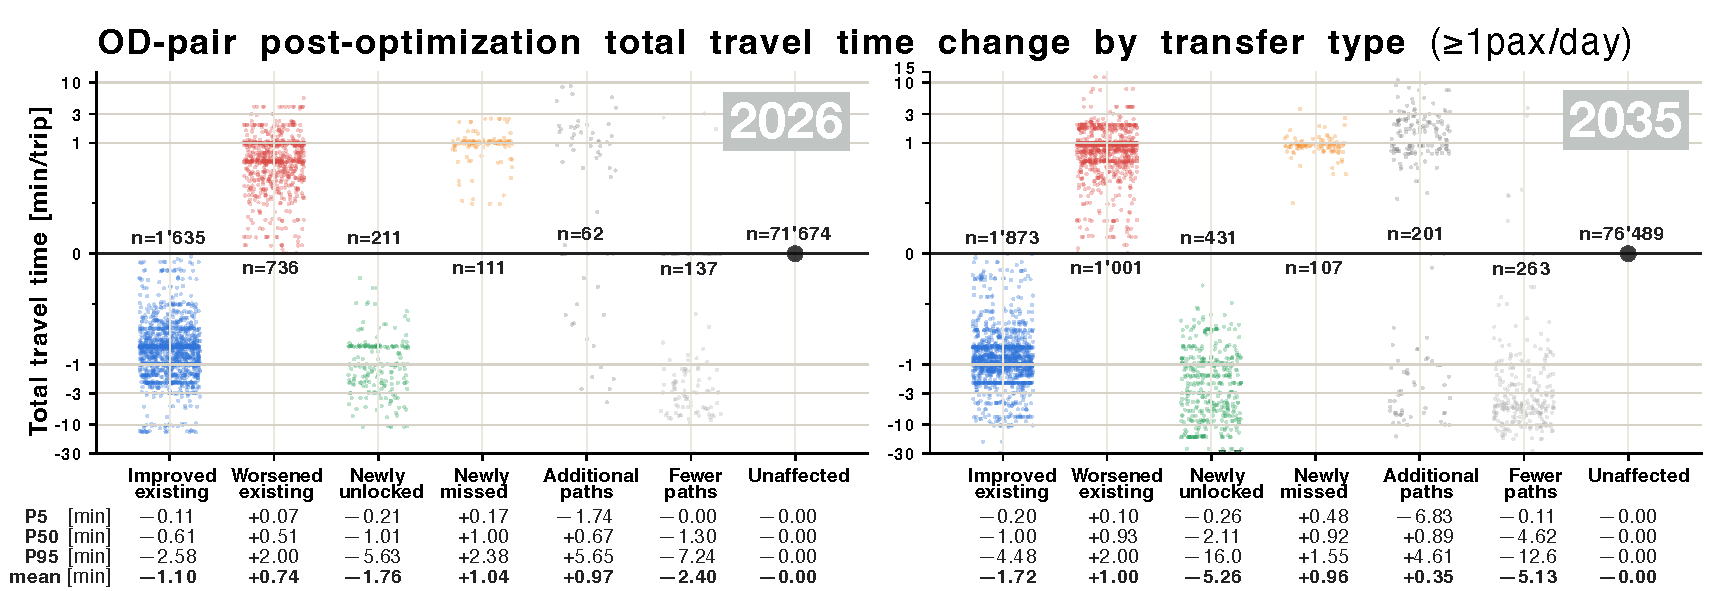
\includegraphics[width=\textwidth]{part2_step3_od_path_change_category_panels_split_paths_scaled.pdf}
    \caption{OD-pair post-optimization total travel-time changes after the final corrected Step~3 timetable, grouped by transfer category or and retained-path change category for all OD pairs with at least 1 passenger per day. The panels separate 2026 and 2035 and show the distribution of per-trip changes within each category, together with category counts, mean, P5, P50 and P95 values. Negative values indicate lower post-optimization travel times.}
    \label{fig:part2-step3-od-path-change-categories}
\end{figure*}

The impact of the accepted line edits is highly selective. Only 3.76\% of positive-demand OD pairs are affected by the altered line timings in 2026 and 3.38\% in 2035. The weighted median OD change therefore remains zero. Nevertheless, the changed set contains important high-flow and transfer-sensitive relations. In the OD pairs with at least 1 pax/day, 2026 contains 1'635 improved-existing relations averaging -1.10 min/trip and 736 worsened-existing relations averaging +0.74 min/trip; newly unlocked relations are fewer, 211, but average -1.76 min/trip. In 2035, 1'873 improved-existing relations average -1.72 min/trip, while 431 newly unlocked relations average -5.26 min/trip. The corresponding newly worsened groups are much smaller: 111 in 2026 and 107 in 2035, averaging +1.04 and +0.96 min/trip. These values clarify why pair counts alone can mislead: the magnitude, demand, and mechanism of changed OD pairs matter jointly.

A further OD-level distinction is whether the number of retained nondominated paths changes. Among OD pairs with at least one passenger per day, 2026 contains 1'635 OD pairs with improved existing transfers averaging -1.10 minutes per trip and 736 OD pairs with worsened existing transfers averaging +0.74 minutes. OD pairs defined by newly unlocked transfers are fewer, 211, but average -1.76 minutes. Newly missed transfers account for only 111 OD pairs, averaging +1.04 minutes. In 2035, there are 1'873 OD pairs with improved existing transfers, averaging -1.72 minutes, while 431 OD pairs with newly unlocked transfers average -5.26 minutes; newly worsened transfers number only 107 and average +0.96 minutes. OD pairs with changed retained-path counts require a separate interpretation: Additional alternatives can appear because a new path becomes attractive, but the dominance-weighted mean can still worsen if shares shift toward a slower retained option. Conversely, fewer retained paths can improve the OD mean when an inferior or less useful option disappears from the nondominated set. The value of a retiming therefore depends on the sign, size, demand, and mechanism of each changed relation.

Spatially, the gains are localized. Ticino is the strongest 2026 origin-canton improvement, while Solothurn leads in 2035; municipality and station-origin effects are more varied still. Reachability and passenger-minute rankings also differ. In 2035, Schlieren reaches 1'192 destinations one minute faster, yet saves only about one quarter of Olten's passenger-minutes because Olten's 101 affected destinations carry higher demand. Segment-load analysis shows fixed demand moving between IC and S-Bahn alternatives in Zurich, between S10 and S20 in Ticino, and between IC61/IC82 and S26/S29. Local event shifts can therefore affect path shares and segment loads far beyond the edited sections.

The OD examples make the mechanism concrete. Olten--Distelberg improves because a one-minute shift turns an infeasible transfer at Aarau into a feasible one by meeting the minimum transfer time; the improvement is not extreme per passenger, but it is valuable because the relation carries meaningful demand. Blankenburg--Le Noirmont, an OD pair with next to 0 demand, illustrates the opposite case: a faster transfer structure can produce a one-hour per-trip improvement for a low-demand relation. These examples justify reporting both saved minutes per trip and passenger-minutes per day. The optimization objective follows the latter, while the former better pinpoints where extreme passenger experiences occur.

The proposed line edits remain traceably linked to their effect on the timetable. Each edit can be traced to a line, a station section, a shift value, a transfer context, and the OD relations affected by the change. This makes the final list of accepted edits usable for a subsequent practical review to confirm whether the proposed small integer-minute shifts are plausible in the local operating context. This future operational review would establish whether they maintain compatibility with available platforms, microscopic track capacity headways, rolling-stock or crew distribution. Due to the minor absolute timing changes inherent to this deliberately non-disruptive model, it can be assumed that a majority of the proposed line edits would be acceptable under these constraints, but further studies are needed.

\section{Discussion II}
The Part II result should be interpreted as a validated national-scale improvement within a restricted search space. The savings are small when averaged over all trips, as expected in an already highly coordinated Swiss clockface timetable, but they are not trivial operationally or economically. A key insight is that suboptimal transfer margins repeated through the day can create passenger-minute losses that are invisible in aggregate timetable descriptions yet recoverable through targeted retiming.

The optimization evaluates a national passenger network after a compact set of local changes. The scale lies in the scenario evaluation: every accepted timetable state is assessed over more than 2 million directed OD pairs per model year, with retained nondominated paths and dominance-based allocation rebuilt after the final scenario. 79 line edits are able to be identified and then linked to broad network effects without globally solving a full national scheduling problem.

The matheuristic design is appropriate because it preserves national passenger detail while avoiding a fully integrated exact formulation and their computational infeasibility for a network of this scale. Benders-type methods and column-generation approaches remain attractive for reduced or otherwise differently formulated instances, and the cited literature demonstrates their value. However, the thesis problem combines national station coverage, millions of directed station pairs, dominance-based path allocation, and full rerouting under fixed demand. Applying an exact integrated PESP/MILP or Benders formulation at this scale would require a new passenger-routing subproblem and strong cuts that fall outside the scope of the thesis, but might justify a worthwhile follow-up investigation. The implemented workflow instead searches interpretable section shifts, verifies candidate compatibility, and validates completed scenarios through full OD rerouting. A main advantage is that every accepted or reversed line edit can be linked to a transfer context, score, compatibility decision, and downstream OD effect. Its limitation is equally clear: no global optimality bound is produced.

Operational limitations remain. Platform occupation, microscopic headways, rolling-stock circulation, crew duties, stochastic delay propagation, fares, and induced demand are outside the model. The accepted edits are therefore passenger-weighted, timetable-validated hypotheses rather than an operationally-validated implementation plan. They are nevertheless a compact shortlist for expert review: 42 active rows in 2026 and 37 in 2035 have already passed structural validation, sequential compatibility checks, and full passenger-network rerouting.

Future research can therefore move in two directions. One direction is operational validation: test the accepted rows against platform occupation, local headways, rolling-stock rotations, crew constraints, and stochastic robustness. The other is methodological: develop incremental or decomposed passenger-routing subproblems that could provide stronger bounds or faster inner-loop evaluation. Benders-style decomposition is promising if passenger-routing subproblems can generate strong cuts, but the thesis results suggest that such a formulation would need to account for changing retained path sets and dominance allocation, not only fixed passenger routes.

\section{Conclusion}
The thesis demonstrates a unified passenger-weighted framework for measuring and improving periodic rail timetables. Part I answers the descriptive question by showing that historical Swiss timetable performance can be reconstructed from timetable tokens, schedule-based routing, OD weighting, and component decomposition. Part II answers the prospective question by showing that small rolling-preserving retimings can reduce national passenger-minutes after full OD rerouting.

The main literature contribution is an integrated application of a matheuristically-determined periodic timetable improvement on a national scale. The work combines accessibility measurement, OD construction, schedule-based routing, dominance allocation, periodic-event retiming, and matheuristic candidate selection across all of Switzerland. It extends passenger-oriented timetable research by demonstrating how a local-search event-retiming matheuristic can produce a fully rerouted, interpretable, and positive network result despite not claiming global optimality. The final finding is therefore that even a highly coordinated clockface railway contains measurable passenger-time potential in small transfer-sensitive retimings, and that potential can be identified when timetable edits are evaluated through the passenger paths they actually create.

The most valuable timetable improvements are not necessarily those with the largest per-trip minute saving, nor those affecting the largest number of OD pairs. They are changes whose passenger-weighted consequences remain positive after all retained paths are rebuilt. A passenger-oriented timetable model must therefore connect local event timing, path feasibility, OD demand, and full-network validation. The thesis demonstrates one way to make that connection for the Swiss clockface railway.

For the literature, the thesis contributes a bridge between measurement and optimization. Accessibility studies often diagnose spatial changes in transport quality; timetabling studies often optimize feasibility and service structure; passenger-assignment studies explain how travellers use a timetable. The work condensed here combines these perspectives. It does not replace exact optimization methods, but it shows that a carefully constrained local-search matheuristic can be useful on larger networks when the objective is to retain full passenger-level routing detail, validate the timetable's feasibility, and adequately quantify post-optimization improvements.
\newpage
\bibliographystyle{IEEEtran}
\bibliography{short_paper_ieee}
\end{document}
